\subsubsection{\stid{1.18} Runtime System for Application-Level Power Steering on Exascale Systems} 

\paragraph{Overview} 
Power remains a critical constraint for Exascale. As we design supercomputers at larger scales, power becomes an expensive and limited resource. Inefficient management of power leads to added operational costs as well as low scientific throughput. Although hardware advances will contribute a certain amount towards achieving high energy efficiency, they will not be sufficient, creating a need for a sophisticated system software approach. Significant advances in software technologies are thus required to ensure that Exascale systems achieve high performance with effective utilization of available power. Distributing available power to nodes while adhering to system, job and node constraints involves complex decision making in software. 

The ECP PowerSteering project is developing a \emph{job-level} power management runtime system that will optimize performance of Exascale scientific applications transparently under power and/or energy constraints. Existing research efforts, including Conductor and Adagio, are being actively integrated into Intel's GEOPM runtime system, an ongoing open source effort led by Intel. This integration expands GEOPM's capabilities with the latest research while providing a production-grade, industry-supported open source solution. By developing new platform plugins, this project also supports upcoming target platforms and paradigms for ECP beyond the Intel architectures, and incorporates task-based programming models such as Legion. By being both configurable and cross-platform, GEOPM will help applications achieve maximum performance under a power constraint. 

This project is essential for ECP because it enables Exascale applications to operate safely with optimal performance under power and energy constraints. This project is also essential for building a sophisticated hierarchical software stack proposed by the ECP Argo and ECP Flux projects. Additionally, the project fulfills an essential need for ECP by enabling vendor and academic collaborations that provide for accelerated adoption of best practices and better interoperability at scale.  By leveraging the GEOPM software developed in this project, compute centers can safely operate under power and energy constraints while maximizing performance and scientific throughput. 


\paragraph{Key Challenges}
Power management in software is challenging due to the dynamic phase behavior of applications, processor manufacturing variability, and the increasing heterogeneity of node-level components. While several scattered research efforts exist, a majority of these efforts are site-specific, require substantial programmer effort, and often result in suboptimal application performance and system throughput. Additionally, these approaches are not production-ready and are not designed to cooperate in an integrated manner. A holistic, generalizable and extensible approach is still missing in the HPC community, and a goal for the ECP PowerSteering project is to provide a solution for this technology gap. 

Another set of challenges come from portability issues. Existing solutions are targeted toward specific Intel microarchitectures as well as programming models. Additionally, some of the existing solutions  violate the specified power budget before reaching a steady state, resulting in power fluctuations as well as unsafe operation. As part of this project, we strive to provide portability as well as safe operation using both hardware-level and application-level information for adaptive configuration selection and critical path analysis.

\paragraph{Solution Strategy}
Our solution is to develop a job-level runtime system (Intel GEOPM) that can operate transparently to user applications, and can also cooperate with HPC resource managers and node-level tools. We are taking a two-pronged approach. First, we are working toward consolidating existing research efforts from the community to develop high-quality plugins for GEOPM that can be deployed at Exascale. In parallel, we are developing new algorithms in GEOPM to address other challenges such as heterogeneity and variation. While GEOPM already provides some baseline algorithms, the existing capabilities are not programmer transparent and not sufficient for Exascale. Our advanced algorithms analyze critical paths of scientific applications transparently, balance power between different components intelligently, and provide mechanisms to capture fine-grained application semantics through Caliper. Additionally, these advanced algorithms will support non-Intel architectures such as IBM/NVIDIA and novel task-based programming models such as Legion. We also intend for GEOPM to be a part of a holistic power management stack that does dynamic, hierarchical power management and works closely with resource managers such as SLURM or Flux.  In order to accomplish portability and smooth integration, we are closely collaborating with ECP Argo and ECP Flux projects, with University of Arizona, and with Intel and IBM. 

\paragraph{Recent Progress}
We achieved two milestones in September 2018. The first was to port GEOPM to a non-Intel architecture. We chose IBM Power9 (Witherspoon) architecture for this, which applies well to the Sierra/Summit systems. We developed a DVFS-based model for Intel GEOPM and leveraged NVIDIA's NVML library to create this port. We also studied the impact of basic telemetry and power capping, and helped identify power-related bugs in IBM OPAL firmware. Currently, we are working on extending \texttt{libvariorum} to support IBM Witherspoon. \texttt{Libvariorum} is a device-agnostic, vendor-neutral power management library which will be integrated into GEOPM in our next milestones. 

The second milestone involved integrating Legion with GEOPM and creating a new benchmark for evaluation. GEOPM calls were placed inside Legion source code because the default model is for a separate GEOPM process to be created, and the GEOPM calls use shared memory to talk to that process. While GEOPM works correctly with Legion in this way, it is unable to provide any benefit with dynamic power balancing due to Legion's inbuilt load balancer. As part of our next milestone, we are researching options to change the default mapper in Legion runtime itself, so we can benefit from power balancing and scheduling power intelligently. Releases were made separately for the two milestones on GitHub. We are now working on testing and evaluation of our framework with the new model and collecting new data on the Quartz cluster at LLNL as well as on \texttt{alehouse}, which is a IBM Power9 node that we purchased for our lab to provide for root and privileged access. 

We established the PowerStack community charter in June 2019, involving collaborators across multiple vendors (Intel, IBM, ARM, HPE, AMD), academic institutions (TU Munich, Univ. Tokyo, Univ. Bologna, Univ. Arizona), and national laboratories (Argonne National Lab).The goal for this team is to design a holistic, flexible and extensible concept of a software stack ecosystem for power management. PowerStack explores hierarchical interfaces at three specific levels: batch job schedulers, job-level runtime systems, node-level managers. Each level will provide options for adaptive management depending on requirements of the supercomputing site under consideration. Site-specific requirements such as cluster-level power bounds, user fairness, or job priorities will be translated as inputs to the job scheduler. The job scheduler will choose plugins to ensure compliance, with the primarily responsibility for managing allocations across multiple users and diverse workloads. Such allocations will serve as inputs to a fine-grained, job-level runtime system to manage specific application ranks, in-turn relying on vendor-agnostic node-level measurement and control mechanisms. The figure below presents an overview of the envisioned PowerStack.

\begin{figure}[t]
	\centering
	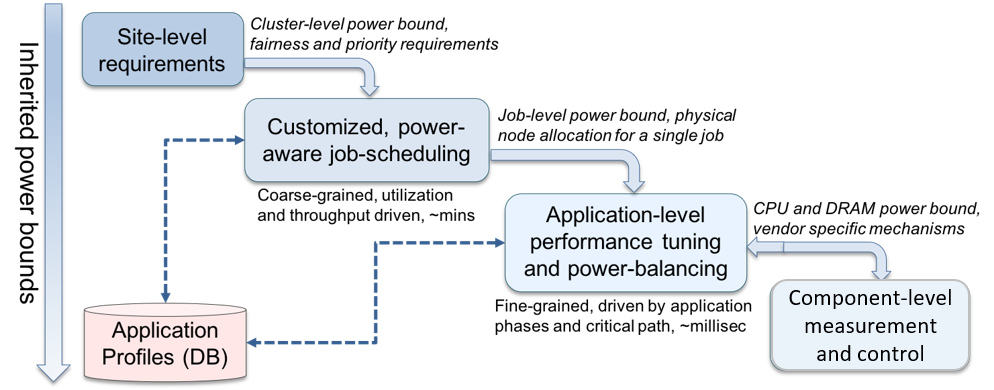
\includegraphics[scale = 0.7]{projects/2.3.1-PMR/2.3.1.19-Argo-PowerSteering/PowerStack_v2.png}
	\caption{Envisioned PowerStack}
	\label{fig:pstack}
\end{figure}

\paragraph{Next Steps}
We will continue our research and development work as planned toward the March 2019 milestones. More specifically, we are migrating to Intel GEOPM's new codebase, working on GPU power capping research, and enabling user-space access to power management on diverse architectures. We also continue to enhance our variation-aware and phase aware model with advanced machine learning and statistical techniques, and are working with Intel on understanding variation data from Theta. In the Legion space, we continue to explore dependency graphs and scheduling of dependency graphs in an intelligent, power-aware manner by creating a new mapper. We are also looking into S3D application code as part of our Legion power model  exploration. Lastly, we are looking into adding Spack support for installing GEOPM. 

\subsubsection{\stid{5.05} Argo} 

\paragraph{Overview} 

The Argo project~\cite{perarnau2017argo} is building portable, open source system software that improves
the performance and scalability and provides increased functionality to
Exascale applications and runtime systems.

We focus on four areas of the OS/R stack where the need from the ECP
applications and facilities is perceived to be the most urgent:
1) support for hierarchical memory;
2) dynamic and hierarchical power management to meet performance
targets;
3) containers for managing resources within a node; and
4) internode interfaces for collectively managing resources across groups
of nodes.


\paragraph{Key Challenges}

Many ECP applications have a complex runtime structure, ranging from in
situ data analysis, through an ensemble of largely independent individual
subjobs, to arbitrarily complex workflow structures~\cite{dreher2017situ}.  At the same time, HPC
hardware complexity increases as well, from deeper memory hierarchies
encompassing on-package DRAM and byte-addressable NVRAM, to heterogeneous
compute resources and performance changing dynamically based on
power/thermal constraints.

To meet the emerging needs of ECP workloads while providing optimal
performance and resilience, the compute, memory, and interconnect resources
must be managed in cooperation with applications and runtime systems; yet
existing resource management solutions lack the necessary capabilities and
vendors are reluctant to innovate in this space in the absence of clear
directions from the community.


\paragraph{Solution Strategy}

Our approach is to augment and optimize for HPC the existing open source
offerings provided by vendors. We are working with ECP applications and
runtime systems to distill the needed new interfaces and to build, test,
and evaluate the newly implemented functionality with ECP workloads.  This
needs to be done in cooperation with facilities, who can provide early
hardware testbeds where the newly implemented functionality can be
demonstrated to show benefits, tested at scale, and matured.  Over the
years we have cultivated an excellent relationship with the vendors
providing HPC platforms because our approach has been to augment and
improve, rather than develop our own OS/R from scratch.  IBM, Cray, and
Intel are eager to integrate the components we develop for ECP that can
help applications.

Our work in each area focuses on the following:

\begin{enumerate}

\item \textbf{Hierarchical memory:} Incorporate NVRAM into the memory hierarchy
using UMap: a user-space \texttt{mmap} replacement for out-of-core data,
leveraging recent \texttt{userfaultfd} mechanism of the Linux kernel for page fault
handling, featuring application-class specific prefetching and eviction
algorithms.  Expose deep DRAM hierarchy by treating high-bandwidth memory
(MCDRAM, HBM) as a scratchpad~\cite{perarnau2016exploring}, managed by the Argonne Memory Library (AML),
which provides applications with asynchronous memory migration
between memory tiers and other convenience mechanisms.

\item \textbf{Power management:}
\emph{PowerStack} explores hierarchical interfaces for power management
at three specific
levels~\cite{Ellsworth:argo,ellsworth_e2sc2016,patki2016,sakamoto2017}: the
global level of batch job schedulers (which we refer to as the Global
Resource Manager or GRM), the enclave level of job-level runtime systems
(open-source solution of Intel GEOPM and the ECP Power Steering project
are being leveraged here), and the node-level through measurement and control
mechanisms integrated with the NRM (described below).
At the node level, we are developing low-level, vendor-neutral
monitoring/controlling capabilities to monitor power/energy consumption,
core temperature and other hardware status~\cite{osti_1353371,zhang2015minimizing}, and control the hardware power
capping and the CPU frequencies. 

\item \textbf{Containers:} Develop a Node Resource Manager (NRM) that leverages
technologies underlying modern container runtimes
(primarily \texttt{cgroups}) to partition resources on compute nodes~\cite{zounmevo2015container},
arbitrating between application components and runtime services.

\item \textbf{Hierarchical resource management:} Develop a set of distributed
services and user-facing interfaces~\cite{perarnau2015distributed} to allow applications and runtimes to
resize, subdivide, and reconfigure their resources inside a job.  Provide
the enclave abstraction: recursive groups of nodes that are managed as a
single entity; those enclaves can then be used to launch new services or to
create subjobs that can communicate with each other.
\end{enumerate}


\paragraph{Recent Progress}

We developed the first stable version of UMap, the user-space memory map
page fault handler for NVRAM.  UMap handler maps application threads'
virtual address ranges to persistent data sets, transparently pages in
active pages and evicts unused pages.  We evaluated the costs and overheads
of various approaches and characterized end-to-end performance for simple
I/O intensive applications.
%
Further work on performance evaluation and capability improvements is
ongoing.  UMap API has been extended to allow for application-specific I/O
strategies.  Read-only support was added to enable the use with released
enterprise versions of the Linux kernel.  UMap now runs on LLNL Sierra.  We
are studying locality-aware eviction and replacement algorithms and are
conducting scaling studies using astronomy application and data.

We developed AML, a memory library for explicit management of deep memory
architectures. Its main feature is a flexible and composable API, allowing
applications to implement algorithms similar to out-of-core for deep
memory.  We provided multiple optimized versions of memory migration
facilities, ranging from a regular copy to a transparent move of memory
pages, using synchronous and asynchronous interfaces and single- and
multithreaded backends.  We validated the initial implementation on Intel's
Knights Landing using a pipelining scheme for stencil applications.  We
also identified interaction points between UMap and AML.  Further
performance and capability improvements are underway.  In particular, we
performed exhaustive studies comparing performance of various approaches
for block-based DGEMM and task-based Cholesky decomposition.

We developed an API between Node Power and Node Resource Manager (NRM),
which in turn allows Global Resource Manager (GRM) to control and monitor
power and other node-local resources.  Additionally, we studied the effect
of power capping on different applications using the NodePower API and
developed power regression models required for a demand-response policy.
We also developed a variation-aware scheduler to address manufacturing
variability under power constraints with Flux infrastructure, and extended
SLURM to support power scheduling plugins.  This was tested on two systems
up to 1,200 nodes and resulted in two publications.  PowerStack is now a
community-wide effort encompassing five industry partners and multiple
academic and research labs across the US, Europe, and Asia.  It enables
prioritization of the critical path, application performance, and
throughput.

We developed the first version of the unified Node Resource Manager.  The
NRM provides high level of control over node resources, including initial
allocation at job launch and dynamic reallocation at the request of the
application and other services.  The initial set of managed resources
includes CPU cores and memory; they can be allocated to application
components via a container abstraction, which is used to describe
partitions of physical resources (to decrease interference), and more.  NRM
integrates dynamic power control using COOLR and libMSR, and provides
support for tracking and reporting of application progress.  Such
functionality is needed by the BSP-oriented power policy, which we are
currently evaluating and scaling up.  Work is also ongoing to support
third-party container technologies such as Docker, Singularity, and
Shifter.  At the job level, we enabled enclave-aware MPI facilities that
can be used to create inter-communicators between MPI jobs launched in
separate enclaves.

On the overall project integration front, we succeeded in creating a first
integrated release, internal for now.  Sources from all the individual
components were pulled into one location.  Testsuites and Spack packages
were created.  We used ChameleonCloud as the first integration platform,
thanks to its capability to provision raw hardware resources.  We also
developed custom CI infrastructure, running on development KNL boxes,
on the ChameleonCloud, and on systems at LLNL.

%\begin{figure}[h]
%\centering
%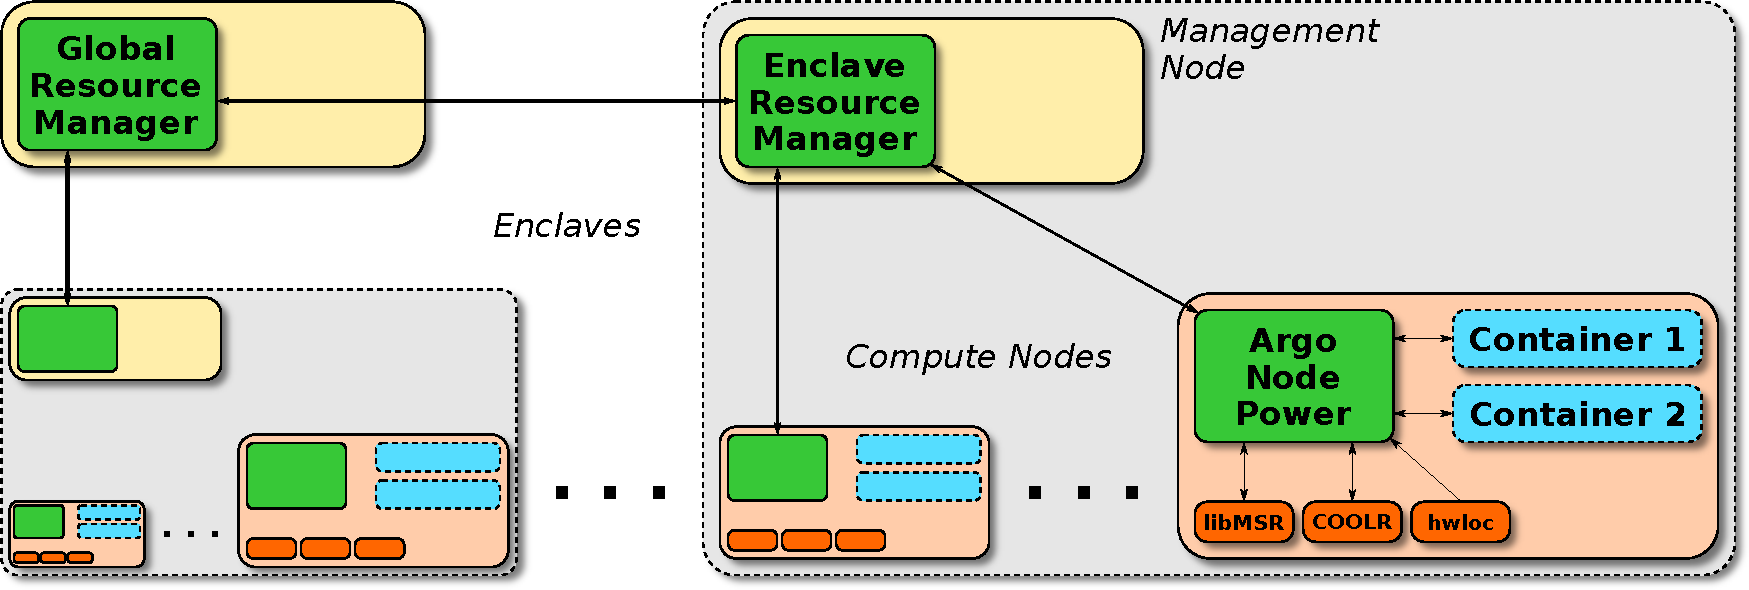
\includegraphics[height=.15\textheight]{projects/2.3.5-Ecosystem/2.3.5.05-Argo/argo-global}\hspace{1em}%
%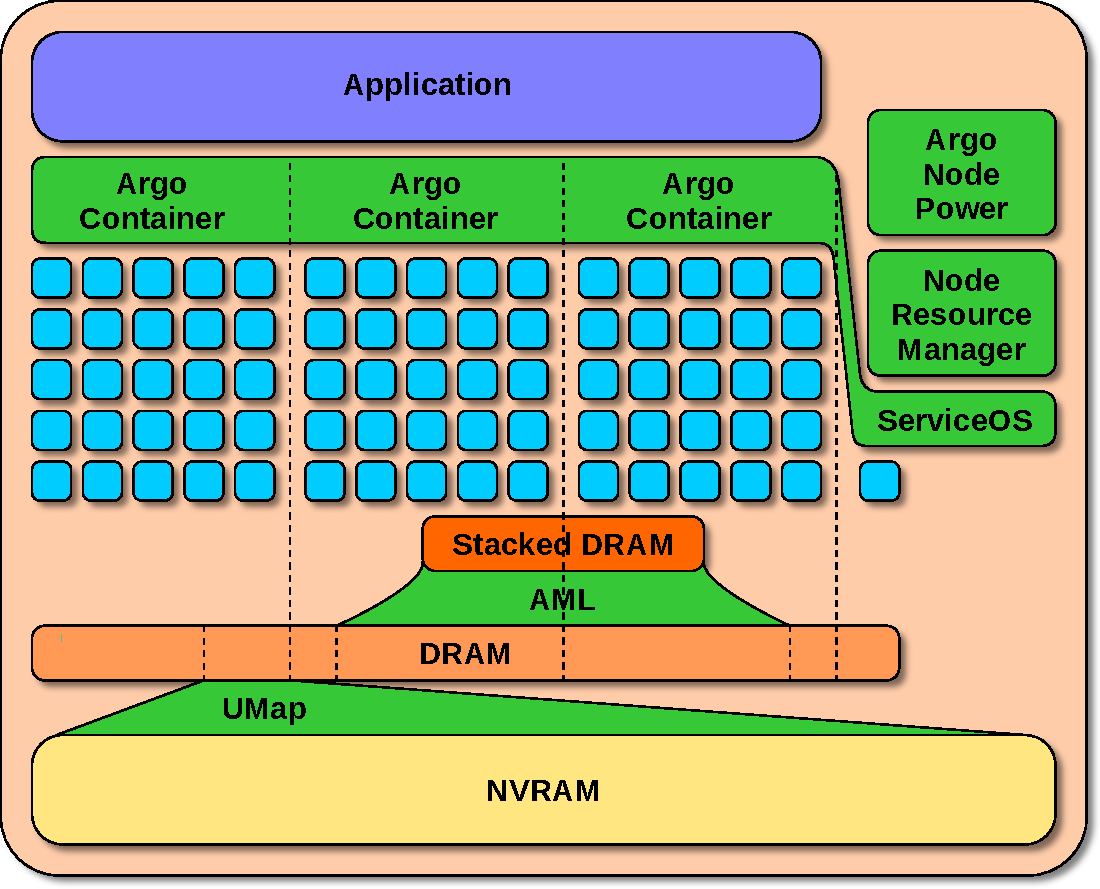
\includegraphics[height=.15\textheight]{projects/2.3.5-Ecosystem/2.3.5.05-Argo/argo-node}
%\caption{Global and node-local components of the Argo software stack and
% interactions between them and the surrounding HPC system components.}
%\end{figure}


\paragraph{Next Steps}

As outlined above, we are actively working on performance and capability
improvements of individual software components and on scaling them up to
leadership-class systems; significant work remains in these areas.

We need to intensify our engagement with ECP applications and runtimes so
that they can benefit from the technologies we have been developing.  We
expect that the newly expanded project team at ANL will enable us to make
significant progress in this area in the near future.

Final software release will take place when the scalability and performance
is validated on a set of relevant ECP workloads.

Looking further into the future, we want to improve resource management for
emerging hardware accelerators, expand dynamic resource management and
placement making it the default, add advanced AI-based autotuning
techniques, use container abstraction to target coupled codes, workflows,
ensembles, and so on.  True byte-addressable NVRAM will enable new,
flexible management and access.
